\section{Sistema \textit{on-line} }

Il sistema di produzione del liquido di dialisi, schematizzato in \figurename~\ref{online}, è gestito automaticamente dalla macchina dializzatrice. Nel caso in esame sono state studiate macchine \textit{Fresenius} $5008s$, commercializzate da \textit{Fresenius Medical Care} AG, Frankfurt, 2005. La macchina dializzatrice, prendendo in ingresso i dati della seduta dialitica, con un algoritmo interno è in grado di miscelare opportunamente il concentrato acido e basico con l'acqua di dialisi, in modo che il liquido dializzante e di diluizione abbiano le portate e le concentrazioni di sodio e bicarbonato prescritte per lo specifico paziente.

\subsection{Sacca acida}
È possibile scegliere fra più sacche acide, diverse fra loro per composizione. Le composizioni delle uniche due sacche utilizzate al centro dialisi sono esposte in Tab.~\ref{tab:acida}. Come si nota, l'unica differenza fra le sacche è data dal \textit{cloruro di potassio}. La scelta della sacca è effettuata dal medico in base alla potassiemia basale del paziente.
\begin{table}[htb]
	\centering
	\caption{Composizione delle sacche acide \textit{Fresenius}. Valori in $mmol/L$}
	\begin{tabular}{lcccccc}
	\toprule 
		\textbf{Codice} & $\mathbf{NaCl}$ & $\mathbf{KCl}$ & $\mathbf{CaCl_2}$ & $\mathbf{MgCl_2}$ & $\mathbf{CH_3COOH}$ & $\mathbf{C_6 H_{12} O_6}$ \\
  \midrule
  	$AX03$ & $4725$ & $90$  & $67,5$   & $22,5$   & $135$      & $249,78$         \\
  	$A161$ & $4725$ & $135$ & $67,5$   & $22,5$   & $135$      & $249,78$         \\
  \bottomrule
\end{tabular}\label{tab:acida}
\end{table}
Conoscendo come si dissociano i sali presenti nella sacca acida, è possibile costruire un'altra tabella in cui compaiono le concentrazioni degli elettroliti e soluti che ci interessa monitorare attraverso il modello numerico. Si tratta di un semplice calcolo stechiometrico il cui risultato è mostrato in Tab.~\ref{tab:acida2}. È evidente che le concentrazioni di questi elettroliti non sono quelle fisiologiche. Il contenuto della sacca acida infatti, prima di essere immesso nel dializzatore, deve prima essere miscelato con la soluzione basica e diluito con l'acqua pura fino a raggiungere i valori prescritti dalla terapia.
\begin{table}[htb]
	\centering
	\caption{Composizione delle sacche acide. Valori in $mmol/L$}
	\begin{tabular}{lcccccc}
	\toprule 
		\textbf{Codice} & $\mathbf{Na^+}$ & $\mathbf{K^+}$ & $\mathbf{Cl^-}$ & $\mathbf{Ca^{++}}$ & $\mathbf{Mg^{++}}$ &  $\mathbf{C_6 H_{12} O_6}$ \\
  \midrule
  	$AX03$ & $4725$ & $90$  & $4995$ & $67,5$    & $22,5$    & $249,78$          \\
  	$A161$ & $4725$ & $135$ & $5040$ & $67,5$    & $22,5$    & $249,78$          \\
  \bottomrule
\end{tabular}\label{tab:acida2}
\end{table}

\subsection{Sacca basica}
La sacca basica (Fresenius biBag\textsuperscript\textregistered) contiene bicarbonato di sodio ($NaHCO_3$) in polvere. Per poterlo utilizzare, la macchina versa sul bicarbonato dell'acqua, la quale viene ripescata dal fondo della sacca quando ormai si è saturata di bicarbonato. Pertanto la concentrazione del liquido basico è quella che assume una soluzione satura di bicarbonato di sodio. I valori di saturazione dell'acqua sono riportati in Tab.~\ref{tab:basica}.
\begin{table}[htb]
	\centering
	\caption{Solubilità di $NaHCO_3$ in acqua}
	\begin{tabular}{lcrrr}
	\toprule 
		\textbf{Temperatura ambiente} & ($^\circ C$) & $0$  & $20$ & $60$  \\
		\textbf{Conc. di saturazione} & ($g/L$)      & $69$ & $96$ & $165$ \\
  \bottomrule
\end{tabular}\label{tab:basica}
\end{table}
Con un interpolazione lineare di questi valori si ottiene che, alla temperatura di circa $25^\circ C$ dell'ambiente in cui il paziente dializza, la concentrazione di sodio ($Na^+$) e dello ione bicarbonato ($HCO_3^-$) contenuti nel liquido basico vale circa $1246$ $mmol/L$.

\subsection{Preparazione del liquido di dialisi}
Il liquido di dialisi e il liquido di sostituzione hanno la stessa composizione di soluti, gestita automaticamente dal software della macchina dializzatrice.
\begin{figure}[htb]
	\centering
		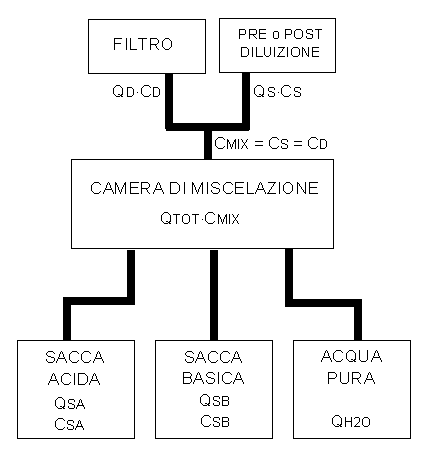
\includegraphics[width=0.4\textwidth]{immagini/on_line_def.eps}
		\caption{Schema del sistema \textit{on-line}. $Q=$ portate, $C^{(s)}=$ concentrazione del soluto $^{(s)}$, $_{SA}=$ sacca acida, $_{SB}=$ sacca basica.}
		\label{online}
\end{figure}
Gli operatori sanitari devono solo impostare sul monitor le concentrazioni prescritte di sodio e bicarbonato, e la macchina, in base alla tipologia della sacca acida e dei parametri fluidodinamici, creerà la giusta miscela. Il sistema di produzione dei fluidi di dialisi è schematizzato in \figurename~\ref{online}. Di questo sistema conosciamo solo alcune quantità mentre altre sono incognite. Queste quantità sono elencate in \tablename~\ref{tab:inc}.
\begin{table}[htb]
\centering
\caption{Dati e incognite del sistema \textit{on-line}.}\label{tab:inc}
\begin{tabularx}{\columnwidth}{lXX}
\toprule
                 & \textbf{dati noti} & \textbf{incognite} \\
\midrule
\textbf{Portate} & $Q_d$, $Q_s$       &     $Q_{sa}$, $Q_{sb}$, $Q_{H_2O}$ \\
\midrule
\textbf{Concentrazioni} &   $C_d^{Na^+}$, $C_d^{HCO_3^-}$, \newline concentrazione di tutti i soluti nelle sacche acida e basica & $C_d^{K^+}$, $C_d^{Cl^-}$, $C_d^{Ca^{++}}$, $C_d^{Mg^{++}}$, \newline fosfato inorganico \\
\bottomrule
\end{tabularx}
\end{table}
Per ricavare le quantità incognite si procede nel modo seguente. Per la conservazione delle portate è possibile scrivere:
\begin{equation}
	Q_{tot} = Q_s + Q_d = Q_{SA} + Q_{SB} + Q_{H_2O}
	\label{eq:Qtot}
\end{equation}
Per la conservazione del bicarbonato, che proviene dalla sola sacca basica, vale:
\begin{equation}
	Q_{SB}\cdot C_{SB}^{(HCO_3^-)} = Q_{tot}\cdot C_{mix}^{(HCO_3^-)}
\end{equation}
dove $C_{mix} = C_d = C_s$ e da cui si ricava l'incognita:
\begin{equation}
	Q_{SB} = \frac{C_{mix}^{(HCO_3^-)}}{C_{SB}^{(HCO_3^-)}}\cdot Q_{tot}
	\label{eq:SB}
\end{equation}
Per la conservazione dello ione sodio, che proviene sia dalla sacca acida che da quella basica, è possibile scrivere:
\begin{equation}
	Q_{tot}\cdot C_{mix}^{(Na^+)} = Q_{SA}\cdot C_{SA}^{(Na^+)} + Q_{SB}\cdot C_{SB}^{(Na^+)}
\end{equation}
da cui si ricava l'incognita:
\begin{equation}
	Q_{SA}= \frac{Q_{tot}\cdot C_{mix}^{(Na^+)} - Q_{SB}\cdot C_{SB}^{(Na^+)}}{C_{SA}^{(Na^+)}}
	\label{eq:SA}
\end{equation}
Scrivendo ora l'equazione di conservazione della massa per il generico soluto $(s)$:
\begin{equation}
	Q_{tot}\cdot C_{mix}^{(s)} = Q_{SA}\cdot C_{SA}^{(s)} + Q_{SB}\cdot C_{SB}^{(s)}
\end{equation}
si può ricavare, per ogni soluto, il valore di concentrazione nel liquido di dialisi:
\begin{equation}
	C_d^{(s)} = C_s^{(s)} = C_{mix}^{(s)} = \frac{Q_{SA}\cdot C_{SA}^{(s)} + Q_{SB}\cdot C_{SB}^{(s)}}{Q_{tot}}
	\label{eq:liquido}
\end{equation}
in cui i valori delle incognite $Q_{SB}$ e $Q_{SA}$ sono rispettivamente forniti dalle equazioni (\ref{eq:SB}) e (\ref{eq:SA}). Per quanto riguarda la portata di acqua $Q_{H_2O}$, che non interessa conoscere ma può essere utile per stimare i consumi, essa può semplicemente essere calcolata per differenza con l'Eq.(\ref{eq:Qtot}).
